\section{Experimental Evaluation}
\label{sec:eval}
The primary evidence comes from direct probes of configured write mappings and fixtures for selected guard and approval branches. A scripted simulator comparison, one injection-twin write, and three language-model episodes provide exploratory context. They do not establish parity between task and direct calls or a complete agent-to-device trace. The scripted comparison uses \texttt{recipe\_trial}, not the task-mediated \texttt{optimization\_explore} sequence in Section~\ref{sec:closed-loop-operation}.

Integrated checks used pre-existing platform and simulator services, generally in benchmark mode, which bypasses step, interval, and hold-window checks for agent or manual writes; ablations removed selected checks, and no cold-start deployment or physical-plant run was performed.

A service response, a simulated readback, and a later process measurement remain distinct throughout this section.

\subsection{Configured Mapping and Integration Checks}
\label{sec:eval-mapping}
Two integrated executions, both seed~42, each passed 77 assertions across 17 phases. Their tool-level loops were scripted; neither run used a language-model agent or constituted an independent deployment. A separate film-line preset check configured five endpoint types and rejected nine selected negative probes. These checks cover preset configuration and direct runtime/API behavior. The scene--protocol matrix below covers structural and value checks in the control direction, not validation of acquisition mappings; timing and hold-window checks are reported separately.

The scene--protocol probes covered 55 configured write-capable endpoints in four simulated scenes over five protocols: Modbus Transmission Control Protocol (TCP), Modbus remote terminal unit (RTU), OPC UA, MQTT, and Hypertext Transfer Protocol (HTTP). Table~\ref{tab:scene-probe-results} gives the scene-level counts. The probe plan specified three requests for interior values, one for the upper boundary, and four for values outside the structural range (the hard engineering range $\mathcal{H}_n$) at each endpoint. All 220 requests with prespecified admissible values received the expected acceptance response; all 219 collected structural-violation requests received the expected rejection, and all 216 available simulator readbacks matched the requested values. One nominal out-of-range candidate lay inside its endpoint's hard range and was filtered before dispatch, so the structural denominator is the 219 collected requests; the single HTTP endpoint provided no readback for its four admissible requests. Because the tested values, the guards, and the expected responses derive from the same configured limits, and the readbacks come from the same simulated stack, these counts show response consistency of the tested mappings, not independent verification. Not every protocol was tested in every scene, so the matrix characterizes selected mappings rather than general protocol interoperability.

\begin{table*}[!t]
\centering
\caption{Configured scene--protocol probes. Counts show prespecified admissible requests receiving the expected acceptance response, collected structural-violation requests receiving the expected rejection, and matching simulator readbacks where the endpoint supports them. The structural denominator is collected requests; one nominal candidate was filtered before dispatch.}
\label{tab:scene-probe-results}
\footnotesize
\setlength{\tabcolsep}{3pt}
\begin{tabularx}{\textwidth}{@{}>{\raggedright\arraybackslash}p{1.55cm}r X r r r@{}}
\toprule
Scene & Configured endpoints & Protocols represented & Accepted probes & Structural rejects & Simulator readbacks \\
\midrule
Injection & 11 & TCP 5; RTU 2; OPC UA 3; MQTT 1 & 44/44 & 44/44 & 44/44 \\
Wastewater & 7 & TCP 1; RTU 3; OPC UA 2; MQTT 1 & 28/28 & 28/28 & 28/28 \\
Annealing & 7 & TCP 3; RTU 2; OPC UA 1; MQTT 1 & 28/28 & 28/28 & 28/28 \\
Biaxial line & 30 & TCP 20; RTU 1; OPC UA 8; HTTP 1 & 120/120 & 119/119 & 116/116 \\
\bottomrule
\end{tabularx}
\end{table*}

\subsection{Exploratory Fixed-Horizon Simulator Contrast}
\label{sec:eval-optimization}
We compared a deterministic bounded setpoint policy with a no-write condition in injection, wastewater, and annealing simulations, using the \texttt{recipe\_trial} route. Candidate adjustments include injection holding pressure and time, wastewater blower and dosing settings, and annealing-zone temperatures and line speed, selected by scene-specific conditions. The target bands were $32.5\pm0.35$~g for part weight, $3.4\pm0.6$~mg/L for dissolved oxygen, and $95\pm6$~HV for hardness, respectively. Each scene used its own fixed horizon (180~s for injection; 240~s for the other scenes), nominal one-second sampling, an independent reset for each arm, and a pre-specified window for the initial process value. Arm order was randomized within each block; paired starts need not have identical process values. The primary outcome was integrated absolute error (IAE), the trapezoidal integral of the absolute deviation from the target-center value over the retained samples; it is not an integral to the nearest band boundary. Internal gaps up to 5~s were linearly interpolated; no extrapolation was made to the nominal window endpoints, and a larger gap invalidated the pair.

After a pilot batch, a later batch of 11 scene--seed blocks was collected; nine met the reset, initial-window, and sampling rules, and two (wastewater seed~45, annealing seed~46) were invalid through 9-s and 6-s no-write sampling gaps. An earlier batch contains a valid, independently reset injection seed-44 block ($\Delta\mathrm{IAE}=193.320$~g\,s; the later batch repeated it with 165.165~g\,s) and failed reset attempts; no batch-selection rule is documented, so the reported subset is exploratory. Every valid block in the later batch had a positive $\Delta\mathrm{IAE}=\mathrm{IAE}_{\mathrm{no\text{-}write}}-\mathrm{IAE}_{\mathrm{scripted}}$. Among valid blocks, every scripted run entered its target band; no no-write run did. Table~\ref{tab:selected-iae} reports per-scene medians and ranges for those nine blocks.

\begin{figure*}[!t]
\centering
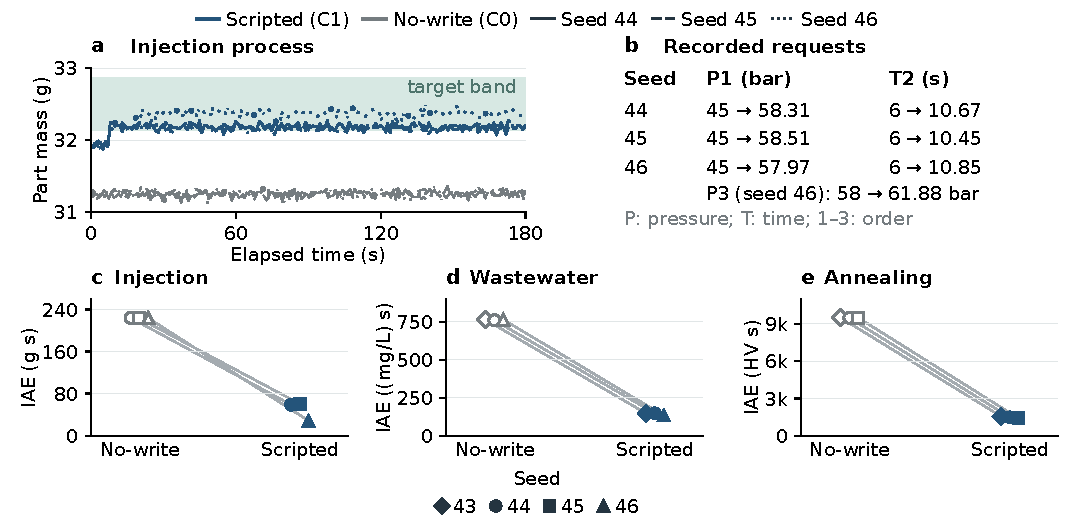
\includegraphics[width=\textwidth]{resources/fig5.pdf}
\caption{Selected exploratory simulator observations. (a) Recorded part-mass samples for the three valid injection scene--seed blocks over the nominal 180~s window; the shaded band is 32.15--32.85~g. Color distinguishes no-write (C0) from the scripted policy (C1), and line style identifies the seed. Sampling gaps beyond 1.5~s appear as breaks and isolated samples as dots; no smoothing is applied. (b) Recorded starting and requested setpoints: P and T denote hold pressure and hold time, and subscripts give request order, not timestamps. These are script records, not independent simulator-device readbacks. (c)--(e) Retained-window IAE for the nine selected scene--seed blocks; markers identify seeds. Each line connects one contrast, and small horizontal offsets only separate overlapping markers. Each scene uses its own scale and reports its native unit multiplied by seconds, so magnitudes are not comparable across scenes. The two blocks invalidated by sampling gaps and the earlier repeated injection block are excluded.}
\label{fig:optimization-trajectory}
\end{figure*}

\begin{table}[!t]
\centering
\caption{Exploratory fixed-horizon simulator contrasts; see text for selection and inference limits. IAE is integrated absolute error to the target-center value. Positive $\Delta$IAE means lower retained-window error under the scripted policy. The Valid column is valid/collected blocks in the later batch.}
\label{tab:selected-iae}
\footnotesize
\setlength{\tabcolsep}{3pt}
\begin{tabular}{@{}lcc@{}}
\toprule
Scene (unit of $\Delta$IAE) & Valid & Median (range) \\
\midrule
Injection (g\,s) & 3/3 & 165.165 (162.535--195.169) \\
Wastewater ((mg/L)\,s) & 3/4 & 615.605 (611.670--630.980) \\
Annealing (HV\,s) & 3/4 & 8000.450 (7930.200--8084.150) \\
\bottomrule
\end{tabular}
\end{table}

The run record's combined SHA-256 matches local copies of the paired-run and policy scripts, but does not identify the executed service image. Without complete service and simulator snapshots, the comparison cannot be reproduced end to end. No-write is a reference for describing the selected blocks, not a competing controller. We tested neither proportional--integral--derivative nor model-predictive control and make no claim about statistical significance, causal improvement, or comparative efficacy.

Fig.~\ref{fig:optimization-trajectory}(a) shows the mass traces of the three valid injection blocks, and (b) tabulates their recorded setpoint requests. Each scripted trace entered the band within 15~s and fluctuated near its lower boundary; no-write traces stayed near their initial values. The three task records report baseline part masses of 31.242, 31.2225, and 31.274~g, respectively; none is necessarily the first sample in the plotted horizon. Seeds~44 and~45 each recorded a pressure then a hold-time request; seed~46 added a further pressure request ($58\rightarrow61.88$~bar) after its hold-time request. The task script's final post-settling means were 32.163, 32.190, and 32.383~g, respectively, within the 32.15--32.85~g band. The starting and requested values in Fig.~\ref{fig:optimization-trajectory}(b) are script records, not independent device readbacks. For seed~46, a prior request to 57.97~bar precedes the later recorded starting value of 58~bar. The archive neither aligns requests with acquisition timestamps nor preserves a per-request server ledger. Fig.~\ref{fig:optimization-trajectory}(c)--(e) compare IAE for the nine selected blocks by scene; Table~\ref{tab:selected-iae} reports the contrasts.

\subsection{Write-Guard and Route Behavior}
\label{sec:eval-ablation}
The guard comparison used direct requests in one simulated scene with a mock driver. Four configurations retained or removed the process-window check (the configured recipe-window limit) and the readback check; Fig.~\ref{fig:guard-approval-results}(a) labels them full guard, no window, no readback, and neither. Hard structural limits stayed active. Each configuration ran three repetitions of four structural, two window, three legal, and three boundary inputs, excluding timed writes. All four rejected 12/12 structural violations and accepted 9/9 legal requests. Each configuration retaining the window check rejected 6/6 window violations (HTTP~400); each without it accepted 6/6 (HTTP~200). Each met its own 9/9 boundary expectations, which changed when the window check was removed. The inputs differed across configurations and the expectations came from the configured limits. This is evidence of the window branch's behavior, not a matched-input effect estimate. The repetitions do not constitute independent trials, HTTP responses do not establish driver dispatch, and this comparison produced no readback mismatch, so it does not assess the readback check.

In a separate follow-up batch, all 110 tested values---two per endpoint, outside the configured recipe window but within structural limits, across the same 55 endpoints---were rejected. In a readback-fault probe, a 230-unit command returned 251 and was graded \texttt{unverified} under a 0.7-unit tolerance; one baseline and one recovery call were \texttt{readback-verified}. Production-mode branch checks rejected one case each for interval, step, node range, recipe window, and hold window, and accepted a legal baseline; separate authorization checks rejected an unbound and a cross-node request and accepted a bound write. These fixtures characterize the selected branches and inputs, not physical-device safety.

The four approval-route calls used scripted decisions and did not follow the full task-mediated sequence; each invoked \texttt{optimization\_explore} directly. The approved call changed the simulated setpoint from 202 to 204.8; the rejected call left 216 unchanged. Two separate calls that bypassed approval changed 202 to 204.8 and 216 to 218.8. Fig.~\ref{fig:guard-approval-results}(b) shows these before and after values. The calls illustrate routing; they are neither a matched ablation nor a test of operator decisions. The route fixtures in this subsection did not exercise post-approval revalidation, approval expiry, \texttt{recipe\_apply} or rollback, in-flight exclusion, or the baseline and product limits of Eq.~(\ref{eq:admission}) in isolation.

\begin{figure*}[!t]
\centering
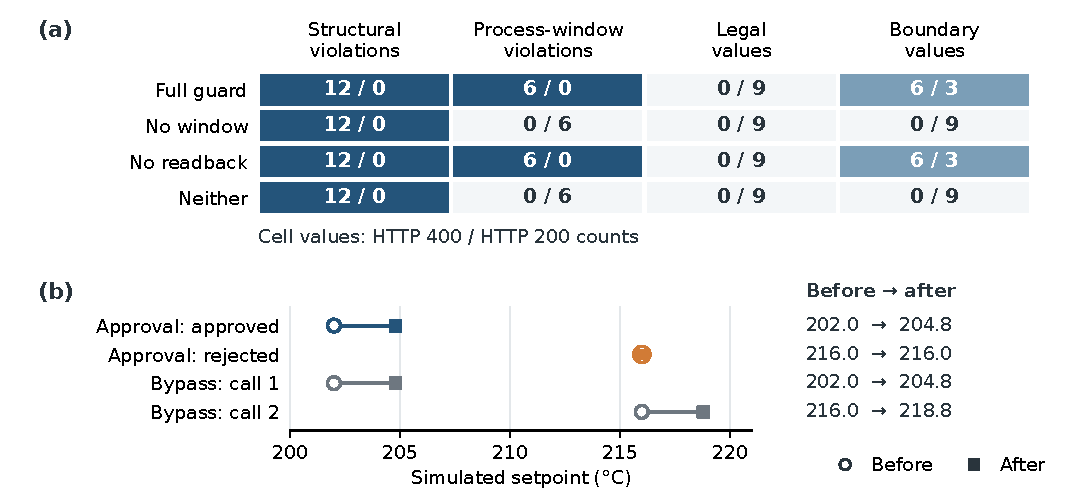
\includegraphics[width=\textwidth]{resources/fig6.pdf}
\caption{Guard-path comparison and scripted approval-route results. (a) Counts of HTTP~400 and HTTP~200 responses for four guard configurations and four request classes, with three repetitions per configuration. Each cell lists rejected/accepted counts, and their sum is the class total; shading represents the proportion of HTTP~400 responses. The specific violation values and boundary expectations differed across configurations. The comparison did not stimulate a readback mismatch. (b) Recorded before and after simulated setpoints for four separate calls; open circles mark before and filled squares after. A scripted proxy supplied the approval decisions, and the bypass calls required no approval. The calls are not matched pairs. HTTP~200 does not establish driver dispatch.}
\label{fig:guard-approval-results}
\end{figure*}

\subsection{Injection-Twin Demonstration}
\label{sec:eval-twin-pilot}
In one acceptance-script run on a PLC-based simulated twin (\texttt{realPlant=false}), a governed write changed holding pressure from 60 to 63.7~bar with matching simulated readback. Three later part-mass samples averaged 32.224~g. The structured and narrative baselines differ (31.503 and 31.508~g, respectively), and neither the raw series nor the complete runtime snapshot was retained. This run illustrates a write and readback, not a process effect.

\subsection{LLM-Driven Simulator Episodes}
\label{sec:eval-agent}
The \texttt{deepseek-flash} endpoint served three injection episodes. The saved worker label was blinded and the served model snapshot was not retained. All three episodes ended \texttt{CANCELED} below the 32.15--32.85~g band, at 31.70, 31.87, and 31.99~g. Each worker trace records one \texttt{recipe\_trial} call to update two setpoints and a response that acknowledged both; approval was automatic, and one episode was flagged for a guard violation. With no row-level server journal retained, these responses do not independently verify driver dispatch, and the episodes do not estimate agent success, approval effects, or physical execution.

